\documentclass[aspectratio=169, 10pt]{beamer}

% --- Packages ---
\usepackage[utf8]{inputenc}
\usepackage{tikz}
\usepackage{pgfplots}
\usepackage{amsmath, amssymb, amsfonts}
\usepackage{mathtools}
\usepackage{booktabs}
\usepackage{array}
\usepackage{bm}
\usepackage{xcolor}
\usetikzlibrary{arrows.meta, calc, positioning, shapes.geometric, decorations.pathreplacing, backgrounds, fit, shadows, patterns, shapes.arrows}
\pgfplotsset{compat=1.17}

% NYU Colors
\definecolor{nyupurple}{RGB}{87,46,140}
\definecolor{nyuheader}{RGB}{172,159,195}
\definecolor{nyufooter}{RGB}{189,178,211}

% Theme
\usetheme{default}
\setbeamertemplate{navigation symbols}{}

% Itemize
\setbeamercolor{itemize item}{fg=nyupurple}
\setbeamercolor{itemize subitem}{fg=nyupurple}
\setbeamercolor{itemize subsubitem}{fg=nyupurple}
\setbeamertemplate{itemize item}{\textbullet}
\setbeamertemplate{itemize subitem}{\textbullet}
\setbeamertemplate{itemize subsubitem}{\textbullet}

% Blocks
\setbeamercolor{block title}{fg=white, bg=nyupurple}
\setbeamercolor{block body}{fg=black, bg=nyuheader!30}
\setbeamercolor{block title alerted}{fg=white, bg=red!70}
\setbeamercolor{block body alerted}{fg=black, bg=red!10}
\setbeamercolor{block title example}{fg=white, bg=green!50!black}
\setbeamercolor{block body example}{fg=black, bg=green!10}

% Diagram colors
\definecolor{darkblue}{RGB}{0,51,102}
\definecolor{brightblue}{RGB}{0,102,204}
\definecolor{lightblue}{RGB}{153,204,255}
\definecolor{darkgreen}{RGB}{0,102,51}
\definecolor{accentred}{RGB}{192,0,0}
\definecolor{accentgreen}{RGB}{0,128,0}
\definecolor{accentorange}{RGB}{255,128,0}

% Commands
\newcommand{\vect}[1]{\boldsymbol{#1}}
\newcommand{\mat}[1]{\mathbf{#1}}

% Header
\makeatletter
\setbeamertemplate{frametitle}{%
    \nointerlineskip%
    \begin{beamercolorbox}[wd=\paperwidth,ht=0.7cm,dp=0.15cm,rightskip=0.5cm]{frametitle}
        \hspace{0.3cm}\usebeamerfont{frametitle}\insertframetitle%
        \hfill%
        \raisebox{0.08cm}{{\bfseries\sffamily\color{nyupurple}NYU}}%
    \end{beamercolorbox}%
}
\makeatother
\setbeamercolor{frametitle}{fg=black, bg=nyuheader}
\setbeamerfont{frametitle}{size=\large}

% Footer
\setbeamertemplate{footline}{%
    \begin{tikzpicture}[remember picture, overlay]
        \fill[nyufooter] ([yshift=0.6cm]current page.south west) rectangle ([xshift=5cm]current page.south east);
        \fill[nyufooter!70] ([yshift=0.6cm, xshift=5cm]current page.south west) rectangle ([xshift=10.5cm]current page.south east);
        \fill[nyufooter!40] ([yshift=0.6cm, xshift=10.5cm]current page.south west) rectangle (current page.south east);
        \node[anchor=west, font=\small] at ([xshift=0.3cm, yshift=0.3cm]current page.south west) {Dr.\ Aliasghar Arab};
        \node[anchor=center, font=\small] at ([yshift=0.3cm]current page.south) {Autonomous Mobile Robots};
        \node[anchor=east, font=\small] at ([xshift=-0.3cm, yshift=0.3cm]current page.south east) {LECTURE 4 -- FALL 2025 \quad \insertframenumber{} / \inserttotalframenumber};
    \end{tikzpicture}%
}

% Title page
\defbeamertemplate*{title page}{customized}[1][]
{
    \begin{tikzpicture}[remember picture, overlay]
        \node[anchor=north east] at ([xshift=-0.8cm, yshift=-0.8cm]current page.north east) {%
            {\bfseries\sffamily\Large\color{nyupurple}NYU}%
            {\sffamily\normalsize\color{black}\ \ TANDON SCHOOL OF ENGINEERING}%
        };
    \end{tikzpicture}
    
    \vspace{2cm}
    \centering
    {\Large\bfseries\inserttitle\par}
    \vspace{0.3cm}
    {\insertsubtitle\par}
    \vspace{1cm}
    {\insertauthor\par}
    \vspace{0.3cm}
    {\small\insertinstitute\par}
    \vspace{0.5cm}
    {\insertdate\par}
}

% Title info
\title{Autonomous Mobile Robots}
\subtitle{Lecture 4: Nonlinear Control Methods}
\author{Dr.\ Aliasghar Arab}
\institute{NYU Tandon School of Engineering}
\date{Fall 2025}

\begin{document}

% ============================================
% TITLE SLIDE
% ============================================
{
\setbeamertemplate{footline}{}
\begin{frame}[plain]
\titlepage
\end{frame}
}

% ============================================
% PART DIVIDER
% ============================================
\begin{frame}
    \begin{center}
        \textcolor{gray}{\Large PART 01}\\[0.5cm]
        {\Huge\textbf{Lecture 4}}\\[0.3cm]
        {\Large\textcolor{darkblue}{Nonlinear Control Methods}}
    \end{center}
\end{frame}

% ============================================
% TOPICS OVERVIEW
% ============================================
\begin{frame}{Topics}
    \begin{columns}
        \begin{column}{0.5\textwidth}
            \begin{enumerate}
                \item Introduction \& Physical Constraints
                \item Vehicle Kinematics \& Equations of Motion
                \item Control \& Perception Fundamentals
                \item \textcolor{darkblue}{\textbf{Nonlinear Control Methods}}
            \end{enumerate}
        \end{column}
        \begin{column}{0.5\textwidth}
            \begin{enumerate}
                \setcounter{enumi}{4}
                \item Advanced MPC + Constraints
                \item Motion Planning Algorithms
                \item Learning-Based Planning \& Control
                \item Industry Standards \& Safety
            \end{enumerate}
        \end{column}
    \end{columns}
\end{frame}

% ============================================
% DESIGNING A CONTROLLER
% ============================================
\begin{frame}{Designing a Controller}
    \begin{itemize}
        \item We are Modelling a \textbf{nonlinear, time-invariant} system:
    \end{itemize}
    
    \begin{columns}
        \begin{column}{0.45\textwidth}
            \begin{block}{System Dynamics}
                \vspace{-0.2cm}
                \[
                \dot{\vect{X}} = f(\vect{X}, u)
                \]
            \end{block}
            
            \vspace{0.2cm}
            Where:
            
            \vspace{0.2cm}
            Robot state = $\vect{X} = \begin{bmatrix} x \\ y \\ \theta \end{bmatrix}$
            
            \vspace{0.3cm}
            $u =$ Control Input $[v, \omega]^T$
        \end{column}
        \begin{column}{0.5\textwidth}
            \centering
            % Fig. 2 - Viewpoint of error coordinate (matching PPT exactly)
            \begin{tikzpicture}[scale=0.75, >=Stealth]
                % Axes
                \draw[->, thick] (-0.3,0) -- (5.5,0) node[right] {X};
                \draw[->, thick] (0,-0.3) -- (0,4.2) node[above] {Y};
                \node at (-0.2,-0.2) {O};
                
                % Current robot position
                \coordinate (current) at (1.8,1.5);
                % Desired robot position
                \coordinate (desired) at (4,3.2);
                
                % Current robot (gray filled rectangle)
                \begin{scope}[shift={(current)}, rotate=25]
                    \fill[gray!30, draw=black] (-0.5,-0.35) rectangle (0.5,0.35);
                    \draw[->, thick, darkblue] (0,0) -- (0.8,0);
                \end{scope}
                
                % Desired robot (gray filled rectangle)
                \begin{scope}[shift={(desired)}, rotate=55]
                    \fill[gray!30, draw=black] (-0.5,-0.35) rectangle (0.5,0.35);
                    \draw[->, thick, darkblue] (0,0) -- (0.8,0);
                \end{scope}
                
                % Position labels
                \draw[dashed, gray] (1.8,0) -- (1.8,1.5);
                \draw[dashed, gray] (0,1.5) -- (1.8,1.5);
                \node at (1.8,-0.3) {$x$};
                \node at (-0.3,1.5) {$y$};
                
                \draw[dashed, gray] (4,0) -- (4,3.2);
                \draw[dashed, gray] (0,3.2) -- (4,3.2);
                \node at (4,-0.3) {$x_d$};
                \node at (-0.3,3.2) {$y_d$};
                
                % Error vectors
                \draw[->, thick, darkred] (current) -- (desired) node[midway, above, sloped] {\small $e_x$};
                
                % Angle labels
                \node at (2.6,1.3) {\small $\theta$};
                \node at (4.8,3.5) {\small $\theta_d$};
                \node at (5.2,3.8) {\small $e_\theta$};
                
                % Caption
                \node at (2.7,-0.8) {\small\textbf{Fig. 2} Viewpoint of error coordinate};
            \end{tikzpicture}
        \end{column}
    \end{columns}
\end{frame}

% ============================================
% ERROR DEFINITION
% ============================================
\begin{frame}{Error Definition}
    \begin{columns}
        \begin{column}{0.5\textwidth}
            \begin{itemize}
                \item Define the \textbf{error vector} as:
            \end{itemize}
            \[
            \vect{e} = \vect{X}_d - \vect{X}
            \]
            
            \vspace{0.2cm}
            Expanding:
            \[
            \vect{e} = \begin{bmatrix} x_d \\ y_d \\ \theta_d \end{bmatrix} - \begin{bmatrix} x \\ y \\ \theta \end{bmatrix}
            \]
            
            \vspace{0.3cm}
            \textbf{Component-wise errors:}
            
            \vspace{0.2cm}
            $e_x = x_d - x$ \quad {\small\textcolor{gray}{(Position error along $x$-axis)}}
            
            \vspace{0.1cm}
            $e_y = y_d - y$ \quad {\small\textcolor{gray}{(Position error along $y$-axis)}}
            
            \vspace{0.1cm}
            $e_\theta = \theta_d - \theta$ \quad {\small\textcolor{gray}{(Heading error)}}
        \end{column}
        \begin{column}{0.45\textwidth}
            \centering
            % Same diagram as slide 4
            \begin{tikzpicture}[scale=0.65, >=Stealth]
                % Axes
                \draw[->, thick] (-0.3,0) -- (5.5,0) node[right] {X};
                \draw[->, thick] (0,-0.3) -- (0,4.2) node[above] {Y};
                \node at (-0.2,-0.2) {O};
                
                % Current robot position
                \coordinate (current) at (1.8,1.5);
                \coordinate (desired) at (4,3.2);
                
                % Current robot
                \begin{scope}[shift={(current)}, rotate=25]
                    \fill[gray!30, draw=black] (-0.5,-0.35) rectangle (0.5,0.35);
                    \draw[->, thick, darkblue] (0,0) -- (0.8,0);
                \end{scope}
                
                % Desired robot
                \begin{scope}[shift={(desired)}, rotate=55]
                    \fill[gray!30, draw=black] (-0.5,-0.35) rectangle (0.5,0.35);
                    \draw[->, thick, darkblue] (0,0) -- (0.8,0);
                \end{scope}
                
                % Position labels
                \draw[dashed, gray] (1.8,0) -- (1.8,1.5);
                \draw[dashed, gray] (0,1.5) -- (1.8,1.5);
                \node at (1.8,-0.3) {$x$};
                \node at (-0.3,1.5) {$y$};
                
                \draw[dashed, gray] (4,0) -- (4,3.2);
                \draw[dashed, gray] (0,3.2) -- (4,3.2);
                \node at (4,-0.3) {$x_d$};
                \node at (-0.3,3.2) {$y_d$};
                
                % Error
                \draw[->, thick, darkred] (current) -- (desired) node[midway, above, sloped] {\small $e_x$};
                
                \node at (2.6,1.3) {\small $\theta$};
                \node at (4.8,3.5) {\small $\theta_d$};
                \node at (5.2,3.8) {\small $e_\theta$};
                
                \node at (2.7,-0.8) {\small\textbf{Fig. 2} Viewpoint of error coordinate};
            \end{tikzpicture}
        \end{column}
    \end{columns}
\end{frame}

% ============================================
% CONTROLLER DESIGN CONSIDERATIONS
% ============================================
\begin{frame}{Things to Focus on While Designing a Controller}
    \begin{center}
        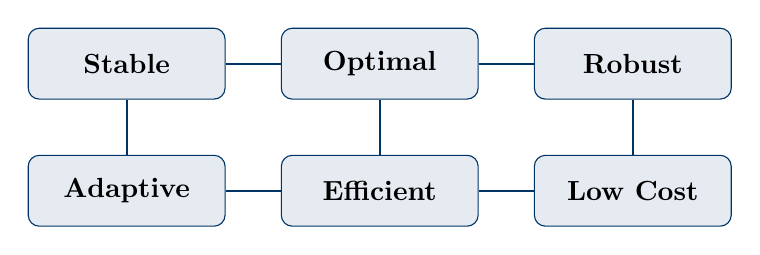
\begin{tikzpicture}[
            node distance=0.7cm,
            box/.style={draw=darkblue, fill=darkblue!10, rounded corners, minimum width=2.5cm, minimum height=0.9cm, align=center, font=\bfseries}
        ]
            \node[box] (stable) {Stable};
            \node[box, right=of stable] (optimal) {Optimal};
            \node[box, right=of optimal] (robust) {Robust};
            \node[box, below=of stable] (adaptive) {Adaptive};
            \node[box, below=of optimal] (efficient) {Efficient};
            \node[box, below=of robust] (lowcost) {Low Cost};
            
            % Connections
            \draw[darkblue, thick] (stable) -- (optimal);
            \draw[darkblue, thick] (optimal) -- (robust);
            \draw[darkblue, thick] (stable) -- (adaptive);
            \draw[darkblue, thick] (optimal) -- (efficient);
            \draw[darkblue, thick] (robust) -- (lowcost);
            \draw[darkblue, thick] (adaptive) -- (efficient);
            \draw[darkblue, thick] (efficient) -- (lowcost);
        \end{tikzpicture}
    \end{center}
    
    \vspace{0.3cm}
    \begin{block}{Key Considerations}
        \begin{itemize}
            \item \textbf{Stability}: Converge to desired state without oscillations
            \item \textbf{Robustness}: Handle model uncertainties and disturbances
            \item \textbf{Optimality}: Minimize energy, time, or tracking error
        \end{itemize}
    \end{block}
\end{frame}

% ============================================
% INDEPENDENT WHEEL CONTROL
% ============================================
\begin{frame}{Independent Wheel Control}
    \begin{columns}
        \begin{column}{0.48\textwidth}
            \textcolor{darkgreen}{\textbf{Pros:}}
            \begin{itemize}
                \item Multiple PI controllers (straightforward loop design)
                \item Works well with ROS kinematic frameworks
                \item Scalable (can extend to more wheels)
                \item Simple at the kinematic level
            \end{itemize}
        \end{column}
        \begin{column}{0.48\textwidth}
            \textcolor{darkred}{\textbf{Cons:}}
            \begin{itemize}
                \item Lacks deeper physical/dynamic understanding
                \item Doesn't capture full robot dynamics
                \item More sensors required (encoders per wheel)
                \item Adds dynamic complexity at higher levels
            \end{itemize}
        \end{column}
    \end{columns}
    
    \vspace{0.4cm}
    \centering
    \begin{tikzpicture}[scale=0.7, >=Stealth,
        block/.style={draw, fill=white, rounded corners, minimum width=1.5cm, minimum height=0.7cm, font=\small}
    ]
        % Left wheel control loop
        \node[block, fill=darkblue!10] (ref1) at (0,0) {$\dot{\phi}_{L,ref}$};
        \node[block, fill=brightgreen!20] (pi1) at (2.5,0) {PI};
        \node[block, fill=lightblue!30] (motor1) at (5,0) {Motor L};
        \node at (7,0) {$\dot{\phi}_L$};
        
        \draw[->] (ref1) -- (pi1);
        \draw[->] (pi1) -- (motor1);
        \draw[->] (motor1) -- (6.5,0);
        \draw[->] (6,0) -- (6,-0.8) -- (1.5,-0.8) -- (1.5,0);
        
        \node at (3.5,-1.3) {\small\textcolor{gray}{(Similar structure for right wheel)}};
    \end{tikzpicture}
\end{frame}

% ============================================
% MOTOR ELECTRICAL DYNAMICS
% ============================================
\begin{frame}{Motor Electrical Dynamics}
    \begin{columns}
        \begin{column}{0.48\textwidth}
            \begin{block}{DC Motor Electrical Equation}
                \vspace{-0.2cm}
                \[
                L\dot{I} + RI = V - K_b \dot{\phi}_m
                \]
            \end{block}
            
            \vspace{0.3cm}
            \textbf{Parameters:}
            \begin{itemize}
                \item $V =$ applied motor voltage
                \item $I =$ current in motor coil
                \item $R =$ coil resistance
                \item $L =$ coil inductance
                \item $K_b \dot{\phi}_m =$ back EMF opposing voltage
            \end{itemize}
        \end{column}
        \begin{column}{0.48\textwidth}
            \centering
            % Motor circuit diagram (matching PPT)
            \begin{tikzpicture}[scale=0.75, >=Stealth]
                % Voltage source
                \draw (0,0) -- (0,1);
                \draw (0,1.5) circle (0.5);
                \node at (0,1.5) {$+$};
                \node at (-0.8,1.5) {\small $V(\phi)$};
                \draw (0,2) -- (0,3);
                
                % Resistor
                \draw (0,3) -- (1,3);
                \draw (1,3) -- (1.2,3.3) -- (1.4,2.7) -- (1.6,3.3) -- (1.8,2.7) -- (2,3.3) -- (2.2,2.7) -- (2.4,3) -- (2.6,3);
                \node at (1.7,3.6) {\small $R$};
                
                % Inductor
                \draw (2.6,3) -- (3,3);
                \draw (3,3) arc (180:0:0.25) arc (180:0:0.25) arc (180:0:0.25);
                \draw (4.5,3) -- (5,3);
                \node at (3.75,3.5) {\small $L$};
                
                % Motor (circle with M)
                \draw (5,3) -- (5,2);
                \draw (5,1.5) circle (0.5);
                \node at (5,1.5) {M};
                \draw (5,1) -- (5,0);
                
                % Return path
                \draw (5,0) -- (0,0);
                
                % Motor shaft and wheel
                \draw[thick] (5.5,1.5) -- (7,1.5);
                
                % Wheel
                \draw[thick] (7,0.5) -- (7,2.5);
                \draw[thick, fill=gray!30] (7,0.8) ellipse (0.15 and 0.4);
                \draw[thick, fill=gray!30] (7,2.2) ellipse (0.15 and 0.4);
                
                % Angular velocity labels
                \draw[->, thick] (6.2,2.2) arc (120:60:0.5);
                \node at (6.5,2.7) {\small $\dot{\phi}_m$};
                
                % Current arrow
                \draw[->, thick, darkred] (0.3,2.8) -- (0.8,2.8);
                \node at (0.55,2.5) {\small $I$};
            \end{tikzpicture}
            
            \vspace{0.2cm}
            {\small\textcolor{gray}{DC Motor Circuit Model}}
        \end{column}
    \end{columns}
\end{frame}

% ============================================
% TORQUE
% ============================================
\begin{frame}{Torque Generation}
    \begin{columns}
        \begin{column}{0.48\textwidth}
            \begin{block}{Motor Torque Equation}
                \vspace{-0.2cm}
                \[
                \boxed{\tau = k_m I}
                \]
            \end{block}
            
            \vspace{0.3cm}
            \textbf{Parameters:}
            \begin{itemize}
                \item $k_m =$ motor torque constant
                \item $I =$ motor current
                \item $\tau =$ generated torque
            \end{itemize}
            
            \vspace{0.3cm}
            \textbf{Key relationship:}
            \[
            \tau \propto I
            \]
            {\small Torque is directly proportional to current}
        \end{column}
        \begin{column}{0.48\textwidth}
            \centering
            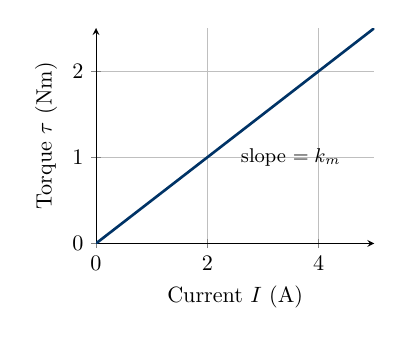
\begin{tikzpicture}[scale=0.8]
                \begin{axis}[
                    xlabel={Current $I$ (A)},
                    ylabel={Torque $\tau$ (Nm)},
                    xmin=0, xmax=5,
                    ymin=0, ymax=2.5,
                    width=6cm, height=5cm,
                    grid=major,
                    axis lines=left,
                ]
                    \addplot[domain=0:5, samples=100, darkblue, very thick] {0.5*x};
                    \node at (axis cs:3.5,1) {\small slope $= k_m$};
                \end{axis}
            \end{tikzpicture}
            
            \vspace{0.2cm}
            {\small\textcolor{gray}{Linear torque-current relationship}}
        \end{column}
    \end{columns}
\end{frame}

% ============================================
% WHEEL MECHANICAL DYNAMICS
% ============================================
\begin{frame}{Wheel Mechanical Dynamics}
    \begin{columns}
        \begin{column}{0.48\textwidth}
            \begin{block}{Rotational Equation of Motion}
                \vspace{-0.2cm}
                \[
                J_w \ddot{\phi} + B_w \dot{\phi} = \tau_m - \tau_L
                \]
            \end{block}
            
            \vspace{0.3cm}
            \textbf{Parameters:}
            \begin{itemize}
                \item $J_w =$ wheel inertia
                \item $B_w \dot{\phi} =$ viscous damping (friction at bearings)
                \item $\tau_m =$ torque from motor
                \item $\tau_L =$ load torque (robot weight, ground resistance)
            \end{itemize}
        \end{column}
        \begin{column}{0.48\textwidth}
            \centering
            \begin{tikzpicture}[scale=0.85, >=Stealth]
                % Wheel
                \draw[very thick, fill=gray!20] (0,0) circle (1.2);
                \draw[very thick, fill=white] (0,0) circle (0.3);
                \fill[darkblue] (0,0) circle (0.12);
                
                % Torque arrows
                \draw[->, darkgreen, very thick] (-0.5,1.5) arc (150:30:0.7);
                \node at (0,1.9) {\small $\tau_m$};
                
                \draw[->, darkred, very thick] (0.5,-1.5) arc (-30:-150:0.7);
                \node at (0,-1.9) {\small $\tau_L$};
                
                % Angular velocity
                \draw[->, darkblue, thick] (1.5,0) arc (0:60:0.5);
                \node at (1.9,0.4) {\small $\dot{\phi}$};
                
                % Ground
                \fill[pattern=north east lines] (-2,-1.3) rectangle (2,-1.5);
                \draw[thick] (-2,-1.3) -- (2,-1.3);
            \end{tikzpicture}
            
            \vspace{0.2cm}
            {\small\textcolor{gray}{Wheel force diagram}}
        \end{column}
    \end{columns}
\end{frame}

% ============================================
% TRANSFER FUNCTION
% ============================================
\begin{frame}{Transfer Function: Voltage to Wheel Speed}
    Combining electrical and mechanical dynamics yields a \textbf{first-order transfer function}:
    
    \vspace{0.5cm}
    \[
    \boxed{\frac{\dot{\phi}(s)}{V(s)} = \frac{r_g \cdot \frac{K_m}{R}}{J_w s + \left(B_w + \frac{K_b K_m}{R}\right)}}
    \]
    
    \vspace{0.5cm}
    \begin{columns}
        \begin{column}{0.48\textwidth}
            \textbf{Parameters:}
            \begin{itemize}
                \item $r_g$ = gear ratio
                \item $R$ = electrical resistance
                \item $J_w$ = wheel inertia
            \end{itemize}
        \end{column}
        \begin{column}{0.48\textwidth}
            \textbf{Motor constants:}
            \begin{itemize}
                \item $B_w$ = mechanical damping
                \item $K_m$ = torque constant
                \item $K_b$ = back-EMF constant
            \end{itemize}
            
            \vspace{0.2cm}
            {\small\textcolor{gray}{Note: Often $K_m \approx K_b$ for DC motors}}
        \end{column}
    \end{columns}
\end{frame}

% ============================================
% WHEEL SPEED CONTROL WITH PID
% ============================================
\begin{frame}{Wheel Speed Control with PID}
    \centering
    % PID Block Diagram (matching PPT exactly)
    \begin{tikzpicture}[scale=0.95, >=Stealth,
        block/.style={draw, fill=white, minimum width=2cm, minimum height=1cm},
        sum/.style={draw, circle, minimum size=0.6cm}
    ]
        % Input
        \node at (-1.2,0) {$\dot{\phi}_c$};
        
        % Sum junction
        \node[sum] (sum) at (1,0) {};
        \draw (sum.north west) -- (sum.south east);
        \draw (sum.north east) -- (sum.south west);
        \node at (0.65,0.4) {\small $+$};
        \node at (0.65,-0.4) {\small $-$};
        
        % PID block
        \node[block, fill=brightgreen!15] (pid) at (4,0) {PID};
        
        % Transfer function block
        \node[block, fill=lightblue!20] (tf) at (7.5,0) {$\dfrac{1}{s+\lambda}$};
        
        % Output
        \node at (10.5,0) {$\dot{\phi}_w$};
        
        % Connections
        \draw[->] (-0.5,0) -- (sum);
        \draw[->] (sum) -- (pid) node[midway, above] {$V_c$};
        \draw[->] (pid) -- (tf);
        \draw[->] (tf) -- (10,0);
        
        % Feedback
        \draw[->] (9,0) -- (9,-1.5) -- (1,-1.5) -- (sum);
    \end{tikzpicture}
    
    \vspace{0.5cm}
    \begin{block}{Control Loop Components}
        \begin{itemize}
            \item $\dot{\phi}_c - \dot{\phi}_w = \text{Error}$
            \item $\dot{\phi}_c =$ Desired wheel speed
            \item $\dfrac{1}{s+\lambda} =$ Approximated wheel + motor dynamics (first-order response)
        \end{itemize}
    \end{block}
\end{frame}

% ============================================
% WHEEL SPEED TO ROBOT MOTION
% ============================================
\begin{frame}{Wheel Speed to Robot Motion}
    \begin{columns}
        \begin{column}{0.5\textwidth}
            \textbf{Robot Pose:}
            \[
            \vect{q} = \begin{bmatrix} x \\ y \\ \theta \end{bmatrix}
            \]
            
            \textbf{Wheel angular velocities:}
            \[
            \dot{\vect{\phi}}_w = \begin{bmatrix} \dot{\phi}_L \\ \dot{\phi}_R \end{bmatrix}
            \]
            
            \vspace{0.3cm}
            \textbf{Kinematic relation:}
            \[
            \boxed{\dot{\vect{q}} = \mat{J}(\vect{q}) \, \dot{\vect{\phi}}_w}
            \]
            
            \vspace{0.2cm}
            $\mat{J}(\vect{q}) =$ Jacobian mapping wheel speeds to body velocities
        \end{column}
        \begin{column}{0.45\textwidth}
            \centering
            \begin{tikzpicture}[scale=0.85, >=Stealth]
                % Robot body (top view)
                \draw[thick, fill=darkblue!15] (-1,-0.5) rectangle (1,0.5);
                
                % Wheels
                \fill[darkblue] (-1,-0.7) rectangle (-0.7,-0.3);
                \fill[darkblue] (0.7,-0.7) rectangle (1,-0.3);
                \fill[darkblue] (-1,0.3) rectangle (-0.7,0.7);
                \fill[darkblue] (0.7,0.3) rectangle (1,0.7);
                
                % Center
                \fill[darkred] (0,0) circle (2pt);
                
                % Wheel labels
                \node at (-0.85,-1) {\small $\dot{\phi}_L$};
                \node at (0.85,-1) {\small $\dot{\phi}_R$};
                
                % Heading
                \draw[->, darkred, thick] (0,0) -- (1.8,0) node[right] {$\theta$};
                
                % Labels
                \node at (0,1.2) {\small Robot pose $\vect{q}$};
            \end{tikzpicture}
            
            \vspace{0.3cm}
            {\small\textcolor{gray}{Differential drive robot}}
        \end{column}
    \end{columns}
\end{frame}

% ============================================
% JACOBIAN FOR DIFFERENTIAL DRIVE
% ============================================
\begin{frame}{Jacobian for Differential Drive}
    \begin{columns}
        \begin{column}{0.5\textwidth}
            \textbf{Kinematic Jacobian:}
            \[
            \mat{J}(\vect{q}) = \frac{r_w}{2} \begin{bmatrix} \cos\theta & \cos\theta \\ \sin\theta & \sin\theta \\ \frac{1}{L} & -\frac{1}{L} \end{bmatrix}
            \]
            
            \vspace{0.5cm}
            \textbf{Parameters:}
            \begin{itemize}
                \item $r_w =$ wheel radius
                \item $L =$ half wheelbase (center to wheel)
            \end{itemize}
        \end{column}
        \begin{column}{0.45\textwidth}
            \centering
            \begin{tikzpicture}[scale=0.85, >=Stealth]
                % Robot body (top view)
                \draw[thick, fill=darkblue!10] (-1,-0.5) rectangle (1,0.5);
                
                % Wheels
                \fill[darkblue] (-1,-0.7) rectangle (-0.7,-0.3);
                \fill[darkblue] (0.7,-0.7) rectangle (1,-0.3);
                \fill[darkblue] (-1,0.3) rectangle (-0.7,0.7);
                \fill[darkblue] (0.7,0.3) rectangle (1,0.7);
                
                % Center
                \fill[darkred] (0,0) circle (2pt);
                
                % Dimensions
                \draw[<->, thick] (0,-1) -- (0.85,-1) node[midway, below] {\small $L$};
                \draw[<->, thick] (-0.85,-1) -- (0,-1) node[midway, below] {\small $L$};
                
                % Wheel radius
                \draw[->, darkgreen] (1.3,0) -- (1.3,0.5) node[midway, right] {\small $r_w$};
                
                % Heading
                \draw[->, darkred, thick] (0,0) -- (1.8,0) node[right] {$\theta$};
            \end{tikzpicture}
        \end{column}
    \end{columns}
\end{frame}

% ============================================
% NONHOLONOMIC CONSTRAINT
% ============================================
\begin{frame}{Nonholonomic Constraint}
    Robot \textbf{cannot move sideways} (no velocity in body-$y$ direction):
    
    \vspace{0.3cm}
    \[
    \boxed{\dot{x}\sin\theta - \dot{y}\cos\theta = 0}
    \]
    
    \vspace{0.2cm}
    Equivalently: $\dot{x}\sin\theta = \dot{y}\cos\theta$
    
    \vspace{0.4cm}
    \begin{columns}
        \begin{column}{0.5\textwidth}
            This \textbf{reduces motion} to two DOFs:
            \[
            \vect{V} = \begin{bmatrix} v \\ \omega \end{bmatrix}
            \]
            \begin{itemize}
                \item $v$ = Linear velocity
                \item $\omega$ = Angular velocity
            \end{itemize}
        \end{column}
        \begin{column}{0.45\textwidth}
            \centering
            \begin{tikzpicture}[scale=0.8, >=Stealth]
                % Robot
                \fill[darkblue!20, draw=darkblue, thick, rounded corners=3pt] (-0.6,-0.4) rectangle (0.6,0.4);
                \fill[darkred] (0,0) circle (2pt);
                
                % Allowed motion
                \draw[->, darkgreen, very thick] (0,0) -- (1.5,0) node[right] {$v$};
                \draw[->, darkblue, thick] (0.3,0.6) arc (90:0:0.6) node[right] {$\omega$};
                
                % Forbidden motion
                \draw[->, darkred, thick, dashed] (0,0) -- (0,1) node[above] {$\times$};
                
                % Labels
                \node at (0,-1) {\small No sideways motion};
            \end{tikzpicture}
        \end{column}
    \end{columns}
\end{frame}

% ============================================
% ROBOT DYNAMIC MODEL
% ============================================
\begin{frame}{Robot Dynamic Model}
    \begin{block}{General Dynamic Equation of Mobile Robot}
        \vspace{-0.2cm}
        \[
        \boxed{\mat{M}(\vect{q})\ddot{\vect{q}} + \mat{C}(\vect{q}, \dot{\vect{q}})\dot{\vect{q}} + \vect{\Delta} = \mat{B}(\vect{q})\vect{\tau}}
        \]
    \end{block}
    
    \vspace{0.4cm}
    \begin{columns}
        \begin{column}{0.48\textwidth}
            \begin{itemize}
                \item $\mat{M}(\vect{q}) =$ inertia (mass) matrix
                \item $\mat{C}(\vect{q}, \dot{\vect{q}})\dot{\vect{q}} =$ Coriolis/centrifugal forces
                \item $\vect{\Delta} =$ disturbances (friction, external forces)
            \end{itemize}
        \end{column}
        \begin{column}{0.48\textwidth}
            \begin{itemize}
                \item $\mat{B}(\vect{q}) =$ input mapping matrix
                \item $\vect{\tau} =$ wheel torques
            \end{itemize}
            
            \vspace{0.3cm}
            {\small\textcolor{gray}{Euler-Lagrange formulation}}
        \end{column}
    \end{columns}
\end{frame}

% ============================================
% TRANSFORMATION RELATIONS
% ============================================
\begin{frame}{Inertia and Coriolis Matrices: Transformation Relations}
    \textbf{Velocity transformation} using the nonholonomic constraint:
    
    \vspace{0.3cm}
    \begin{columns}
        \begin{column}{0.5\textwidth}
            \[
            \dot{\vect{q}} = \mat{T}_v \vect{V}
            \]
            
            \[
            \ddot{\vect{q}} = \dot{\mat{T}}_v \vect{V} + \mat{T}_v \dot{\vect{V}}
            \]
            
            \vspace{0.3cm}
            where $\vect{V} = [v, \omega]^T$
        \end{column}
        \begin{column}{0.45\textwidth}
            \textbf{Transformation matrix:}
            \[
            \mat{T}_v(\theta) = \begin{bmatrix} \cos\theta & 0 \\ \sin\theta & 0 \\ 0 & 1 \end{bmatrix}
            \]
        \end{column}
    \end{columns}
    
    \vspace{0.5cm}
    {\small This maps the 2D velocity space $\vect{V}$ to the 3D configuration space derivative $\dot{\vect{q}}$.}
\end{frame}

% ============================================
% INERTIA AND CORIOLIS MATRICES - EXPLICIT
% ============================================
\begin{frame}{Inertia and Coriolis Matrices}
    \textbf{Inertia Matrix:}
    \[
    \mat{M}(\vect{q}) = \begin{bmatrix} m & 0 & -md\sin\theta \\ 0 & m & md\cos\theta \\ -md\sin\theta & md\cos\theta & I_{zz} \end{bmatrix}
    \]
    
    \vspace{0.4cm}
    \textbf{Coriolis Matrix:}
    \[
    \mat{C}(\vect{q}, \dot{\vect{q}}) = \begin{bmatrix} 0 & 0 & -md\dot{\theta}\cos\theta \\ 0 & 0 & -md\dot{\theta}\sin\theta \\ 0 & 0 & 0 \end{bmatrix}
    \]
    
    \vspace{0.3cm}
    {\small\textcolor{gray}{$m$ = total mass, $d$ = offset from center to CoM, $I_{zz}$ = moment of inertia}}
\end{frame}

% ============================================
% PROPERTY OF ROBOT DYNAMICS
% ============================================
\begin{frame}{Property of Robot Dynamics: Skew Symmetry}
    \begin{block}{Skew-Symmetric Property}
        The matrix $\dot{\mat{M}}(\vect{q}) - 2\mat{C}(\vect{q}, \dot{\vect{q}})$ is \textbf{skew-symmetric}.
    \end{block}
    
    \vspace{0.3cm}
    For a skew-symmetric matrix $\mat{A}$:
    \[
    \mat{A} = -\mat{A}^T \qquad \Rightarrow \qquad \vect{x}^T \mat{A} \vect{x} = 0
    \]
    
    \vspace{0.4cm}
    \textbf{Importance:}
    \begin{itemize}
        \item Guarantees \textbf{energy conservation} in robot dynamics
        \item Essential for proving \textbf{stability} using Lyapunov methods
        \item Exploited in passivity-based control design
    \end{itemize}
\end{frame}

% ============================================
% DERIVING VELOCITY-SPACE DYNAMICS
% ============================================
\begin{frame}{Finding the EOM of the Robot}
    \textbf{Configuration-space dynamics:}
    \[
    \mat{M}(\vect{q})\ddot{\vect{q}} + \mat{C}(\vect{q}, \dot{\vect{q}})\dot{\vect{q}} + \vect{\Delta} = \mat{B}(\vect{q})\vect{\tau}
    \]
    
    \vspace{0.3cm}
    \textbf{Substitute} transformation $\dot{\vect{q}} = \mat{T}_v \vect{V}$ and $\ddot{\vect{q}} = \dot{\mat{T}}_v \vect{V} + \mat{T}_v \dot{\vect{V}}$:
    \[
    \mat{M}(\vect{q})\left(\mat{T}_v \dot{\vect{V}} + \dot{\mat{T}}_v \vect{V}\right) + \mat{C}(\vect{q}, \dot{\vect{q}})\mat{T}_v \vect{V} + \vect{\Delta} = \mat{B}\vect{\tau}
    \]
    
    \vspace{0.3cm}
    \textbf{Velocity-space dynamics:}
    \[
    \boxed{\bar{\mat{M}}(\vect{q})\dot{\vect{V}} + \bar{\mat{C}}(\vect{q}, \dot{\vect{q}})\vect{V} + \bar{\vect{\Delta}} = \bar{\mat{B}}(\vect{q})\vect{\tau}}
    \]
\end{frame}

% ============================================
% VELOCITY-SPACE DYNAMIC PARAMETERS
% ============================================
\begin{frame}{Final Velocity-Space Dynamics}
    \textbf{Transformed matrices:}
    
    \vspace{0.3cm}
    \begin{align*}
        \bar{\mat{M}}(\vect{q}) &= \mat{T}_v^T \mat{M}(\vect{q}) \mat{T}_v \\[0.3cm]
        \bar{\mat{C}}(\vect{q}, \dot{\vect{q}}) &= \mat{T}_v^T \left[\mat{M}(\vect{q})\dot{\mat{T}}_v + \mat{C}(\vect{q}, \dot{\vect{q}})\mat{T}_v\right] \\[0.3cm]
        \bar{\mat{B}} &= \mat{T}_v^T \mat{B}(\vect{q}) \\[0.3cm]
        \bar{\vect{\Delta}} &= \mat{T}_v^T \vect{\Delta}
    \end{align*}
    
    \vspace{0.3cm}
    {\small These 2$\times$2 matrices are much simpler than the original 3$\times$3 matrices!}
\end{frame}

% ============================================
% COMMAND VELOCITY
% ============================================
\begin{frame}{Command Velocity $\vect{V}_c$}
    \textbf{Kinematic control law} for trajectory tracking:
    
    \vspace{0.3cm}
    \[
    \vect{V}_c = \begin{bmatrix} v_d \cos(e_\theta) + k_x e_x \\ \omega_d + k_y v_d e_y + k_\theta v_d \sin(e_\theta) \end{bmatrix}
    \]
    
    \vspace{0.3cm}
    \begin{columns}
        \begin{column}{0.5\textwidth}
            \textbf{Inputs:}
            \begin{itemize}
                \item $\vect{q}_d = [x_d, y_d, \theta_d]^T$ -- Desired pose
                \item $v_d, \omega_d$ -- Desired velocities
            \end{itemize}
        \end{column}
        \begin{column}{0.45\textwidth}
            \textbf{Gains:} $k_x, k_y, k_\theta > 0$
        \end{column}
    \end{columns}
    
    \vspace{0.4cm}
    \begin{alertblock}{Note}
        This controller is for \textbf{trajectory tracking}, not set-point regulation.
    \end{alertblock}
\end{frame}

% ============================================
% OVERALL CONTROL STRUCTURE
% ============================================
\begin{frame}{Overall Control Structure}
    \centering
    % Overall control structure block diagram (matching PPT)
    \begin{tikzpicture}[scale=0.62, >=Stealth,
        block/.style={draw, fill=white, minimum width=2.8cm, minimum height=0.9cm, font=\small},
        smallblock/.style={draw, fill=white, minimum width=1.2cm, minimum height=0.9cm, font=\small},
        sum/.style={draw, circle, minimum size=0.5cm}
    ]
        % Input
        \node at (-1.8,0) {\small $(q_d, v_d)$};
        
        % Kinematic Controller
        \node[block, fill=brightgreen!15] (kin) at (2,0) {Kinematic Controller};
        
        % Sum junction
        \node[sum] (sum) at (5.2,0) {};
        \draw (sum.north west) -- (sum.south east);
        \draw (sum.north east) -- (sum.south west);
        
        % Dynamic Controller
        \node[block, fill=lightblue!20] (dyn) at (9,0) {2nd-Wheel Dynamic Controller};
        
        % Robot
        \node[smallblock, fill=darkorange!15] (robot) at (12.5,0) {Robot};
        
        % Integrator
        \node[smallblock] (int) at (15,0) {$\frac{1}{s}$};
        
        % Output
        \node at (17,0) {\small $q$};
        
        % V_c label
        \node at (3.8,0.5) {\small $V_c$};
        
        % q_dot label
        \node at (13.7,0.5) {\small $\dot{q}$};
        
        % Connections
        \draw[->] (-0.8,0) -- (kin);
        \draw[->] (kin) -- (sum);
        \draw[->] (sum) -- (dyn);
        \draw[->] (dyn) -- (robot);
        \draw[->] (robot) -- (int);
        \draw[->] (int) -- (16.5,0);
        
        % Feedback through Transform
        \node[block] (trans) at (9,-2.5) {Transform};
        \draw[->] (16,0) -- (16,-2.5) -- (trans);
        \draw[->] (trans) -- (5.2,-2.5) -- (sum);
    \end{tikzpicture}
    
    \vspace{0.4cm}
    \begin{block}{Control Architecture}
        \begin{itemize}
            \item \textbf{Kinematic Controller} $\rightarrow$ computes command velocity $V_c$ from tracking errors
            \item \textbf{Dynamic Controller} $\rightarrow$ converts $V_c$ into wheel torques $\tau$
            \item \textbf{Robot + EOM} $\rightarrow$ updates motion states $(q, \dot{q})$
            \item \textbf{Feedback transform} $\rightarrow$ converts states to error signals
        \end{itemize}
    \end{block}
\end{frame}

% ============================================
% FEEDBACK LINEARIZATION
% ============================================
\begin{frame}{Feedback Linearization: Motivation}
    \textbf{Robot velocity dynamics:}
    \[
    \bar{\mat{M}}(\vect{q})\dot{\vect{V}} + \bar{\mat{C}}(\vect{q}, \dot{\vect{q}})\vect{V} + \bar{\vect{\Delta}} = \bar{\mat{B}}\vect{\tau}
    \]
    
    \vspace{0.3cm}
    \textbf{Goal:} Design $\vect{\tau}$ such that robot velocity $\vect{V}$ tracks desired $\vect{V}_c(t)$.
    
    \vspace{0.5cm}
    \begin{block}{General Nonlinear System}
        \[
        \dot{\vect{x}} = f(\vect{x}, \vect{u})
        \]
        Feedback linearization transforms this into a \textbf{linear} closed-loop system.
    \end{block}
\end{frame}

% ============================================
% LINEARIZATION IDEA
% ============================================
\begin{frame}{Linearization Idea (General System)}
    \textbf{Nonlinear system:} $\dot{x} = f(x) + b(x)u$
    
    \vspace{0.3cm}
    \textbf{Choose control law:}
    \[
    u = b^{-1}\left[-f(x) + \dot{x}_d + k(x_d - x)\right]
    \]
    
    \vspace{0.3cm}
    \textbf{Substituting into the system:}
    \[
    \dot{x} = \dot{x}_d + k(x_d - x)
    \]
    
    \vspace{0.3cm}
    \textbf{Error dynamics:} Define $e = x_d - x$
    \[
    \boxed{\dot{e} + ke = 0}
    \]
    
    {\small Linear, exponentially stable error dynamics with rate $k > 0$.}
\end{frame}

% ============================================
% CONTROL LAW FOR THE ROBOT
% ============================================
\begin{frame}{Control Law for the Robot}
    \textbf{Apply feedback linearization} to velocity-space dynamics.
    
    \vspace{0.2cm}
    \textbf{Velocity-space EOM:}
    \[
    \bar{\mat{M}}(\vect{q})\dot{\vect{V}} + \bar{\mat{C}}(\vect{q}, \dot{\vect{q}})\vect{V} + \bar{\vect{\Delta}} = \bar{\mat{B}}\vect{\tau} \quad \hookrightarrow (1)
    \]
    
    \vspace{0.2cm}
    \textbf{Chosen input torque:}
    \[
    \vect{\tau} = \bar{\mat{B}}^{-1}\left[\bar{\mat{M}}(\vect{q})\dot{\vect{V}}_c + \bar{\mat{C}}(\vect{q}, \dot{\vect{q}})\vect{V} + \tilde{\vect{\Delta}} + \mat{K}(\vect{V}_c - \vect{V})\right] \quad \hookrightarrow (2)
    \]
    
    \vspace{0.3cm}
    \textbf{Substituting (2) into (1):}
    \[
    \bar{\mat{M}}(\vect{q})(\dot{\vect{V}}_c - \dot{\vect{V}}) + \mat{K}(\vect{V}_c - \vect{V}) = \tilde{\vect{\Delta}} - \bar{\vect{\Delta}}
    \]
\end{frame}

% ============================================
% CLOSED-LOOP ERROR DYNAMICS
% ============================================
\begin{frame}{Closed-Loop Error Dynamics}
    \[
    \bar{\mat{M}}(\vect{q})(\dot{\vect{V}}_c - \dot{\vect{V}}) + \mat{K}(\vect{V}_c - \vect{V}) = \tilde{\vect{\Delta}} - \bar{\vect{\Delta}}
    \]
    
    \vspace{0.3cm}
    \textbf{Define velocity error:} $\vect{e}_v = \vect{V}_c - \vect{V}$
    
    \vspace{0.3cm}
    \textbf{Error dynamics:}
    \[
    \boxed{\dot{\vect{e}}_v + \mat{K}'\vect{e}_v = \vect{\delta}(t)}
    \]
    
    where:
    \begin{align*}
        \mat{K}' &= \bar{\mat{M}}(\vect{q})^{-1}\mat{K} \\
        \vect{\delta}(t) &= \bar{\mat{M}}(\vect{q})^{-1}(\tilde{\vect{\Delta}} - \bar{\vect{\Delta}})
    \end{align*}
    
    {\small If $\tilde{\vect{\Delta}} = \bar{\vect{\Delta}}$ (perfect estimation), error converges exponentially to zero.}
\end{frame}

% ============================================
% SECOND-ORDER ERROR DYNAMICS
% ============================================
\begin{frame}{Second-Order Error Dynamics}
    For \textbf{position tracking}, consider position error $\vect{e}$:
    
    \vspace{0.3cm}
    \[
    \boxed{\ddot{\vect{e}} + k_d \dot{\vect{e}} + k_p \vect{e} = 0}
    \]
    
    \vspace{0.3cm}
    \textbf{Characteristic equation:}
    \[
    s^2 + 2\zeta\omega_n s + \omega_n^2 = 0
    \]
    
    \vspace{0.3cm}
    \begin{columns}
        \begin{column}{0.5\textwidth}
            \textbf{Standard form:}
            \begin{itemize}
                \item $k_p = \omega_n^2$ (natural frequency)
                \item $k_d = 2\zeta\omega_n$ (damping)
            \end{itemize}
        \end{column}
        \begin{column}{0.45\textwidth}
            \textbf{Design choice:}
            \begin{itemize}
                \item $\zeta = 1$ for critical damping
                \item $\omega_n$ sets convergence rate
            \end{itemize}
        \end{column}
    \end{columns}
\end{frame}

% ============================================
% SET-POINT CONTROL
% ============================================
\begin{frame}{Set-Point Control: Virtual Output}
    \textbf{Goal:} Stabilize robot at desired position $(x_d, y_d)$
    
    Instead of directly controlling $(x, y, \theta)$, define a \textbf{virtual output}:
    
    \begin{columns}
        \begin{column}{0.42\textwidth}
            \[
            \vect{Y} = \begin{bmatrix} x + \alpha\cos\theta \\ y + \alpha\sin\theta \end{bmatrix}
            \]
            
            \vspace{0.2cm}
            Point at distance $\alpha$ ahead of robot center.
            
            \vspace{0.3cm}
            \[
            \mat{M}\ddot{\vect{q}} + \mat{C}\dot{\vect{q}} + \vect{\Delta} = \mat{B}\vect{\tau}
            \]
            
            \[
            \bar{\mat{M}}\dot{\vect{V}} + \bar{\mat{C}}\vect{V} + \bar{\vect{\Delta}} = \mat{B}\vect{\tau}
            \]
        \end{column}
        \begin{column}{0.55\textwidth}
            \centering
            % Robot diagram with virtual output point (matching PPT slide 32)
            \begin{tikzpicture}[scale=0.65, >=Stealth]
                % Axes
                \draw[->, thick] (-0.5,0) -- (5,0) node[right] {X};
                \draw[->, thick] (0,-0.5) -- (0,4) node[above] {Y};
                \node at (-0.2,-0.2) {O};
                
                % Robot body (rotated rectangle)
                \begin{scope}[shift={(2.5,2)}, rotate=30]
                    % Body
                    \draw[thick] (-0.8,-0.5) rectangle (0.8,0.5);
                    
                    % Wheels
                    \fill[black] (-0.7,-0.7) rectangle (-0.5,-0.5);
                    \fill[black] (-0.7,0.5) rectangle (-0.5,0.7);
                    \fill[black] (0.5,-0.7) rectangle (0.7,-0.5);
                    \fill[black] (0.5,0.5) rectangle (0.7,0.7);
                    
                    % Center point C
                    \fill[darkblue] (0,0) circle (2pt);
                    \node at (0.3,0.2) {\small $C$};
                    
                    % Virtual point at distance alpha
                    \draw[dashed, darkred] (0,0) -- (1.2,0);
                    \fill[darkred] (1.2,0) circle (2pt);
                    \node at (1.4,0.2) {\small $d$};
                    
                    % Heading direction
                    \draw[->, thick, darkblue] (0,0) -- (1.8,0);
                    
                    % Wheelbase labels
                    \draw[<->, thin] (-0.6,-1) -- (0.6,-1);
                    \node at (0,-1.3) {\small $2b$};
                    
                    % Wheel radius
                    \draw[<->, thin] (1,-0.6) -- (1,0.6);
                    \node at (1.4,0) {\small $2r$};
                \end{scope}
                
                % Position labels
                \draw[dashed, gray] (2.5,0) -- (2.5,2);
                \draw[dashed, gray] (0,2) -- (2.5,2);
                \node at (2.5,-0.3) {\small $x$};
                \node at (-0.3,2) {\small $y$};
                
                % Y_r label
                \node at (-0.3,3) {\small $Y_r$};
                
                % Angle theta
                \draw[->] (3.5,2) arc (0:30:1);
                \node at (3.9,2.3) {\small $\theta$};
            \end{tikzpicture}
        \end{column}
    \end{columns}
\end{frame}

% ============================================
% SET-POINT CONTROL (continued)
% ============================================
\begin{frame}{Set-Point Control: Virtual Output Dynamics}
    \textbf{Time derivatives of virtual output:}
    \[
    \dot{\vect{Y}} = \mat{\Lambda}\vect{V} \qquad \ddot{\vect{Y}} = \dot{\mat{\Lambda}}\vect{V} + \mat{\Lambda}\dot{\vect{V}}
    \]
    
    \vspace{0.3cm}
    \textbf{Decoupling matrix:}
    \[
    \mat{\Lambda} = \begin{bmatrix} \cos\theta & -\alpha\sin\theta \\ \sin\theta & \alpha\cos\theta \end{bmatrix}
    \]
    
    \vspace{0.4cm}
    \begin{alertblock}{Important}
        $\mat{\Lambda}$ is invertible when $\alpha \neq 0$, enabling full control of the virtual output.
    \end{alertblock}
\end{frame}

% ============================================
% CONTROL LAW FOR SET-POINT
% ============================================
\begin{frame}{Set-Point Control Law}
    \textbf{Transformed dynamics} in terms of virtual output:
    \[
    \tilde{\mat{M}}\ddot{\vect{Y}} + \tilde{\mat{C}}\dot{\vect{Y}} + \tilde{\vect{\Delta}} = \tilde{\mat{B}}\vect{\tau}
    \]
    
    where $\tilde{\mat{M}}, \tilde{\mat{C}}, \tilde{\vect{\Delta}}, \tilde{\mat{B}}$ are transformed using $\mat{\Lambda}$.
    
    \vspace{0.5cm}
    \textbf{PD control law with feedforward:}
    \[
    \boxed{\vect{\tau} = \tilde{\mat{B}}^{-1}\left[\tilde{\mat{M}}\ddot{\vect{Y}}_d + \tilde{\mat{C}}\dot{\vect{Y}} + \tilde{\vect{\Delta}} + k_d(\dot{\vect{Y}}_d - \dot{\vect{Y}}) + k_p(\vect{Y}_d - \vect{Y})\right]}
    \]
    
    \vspace{0.3cm}
    For set-point control: $\vect{Y}_d = \text{const}$, so $\dot{\vect{Y}}_d = \ddot{\vect{Y}}_d = 0$.
\end{frame}

% ============================================
% CLOSED-LOOP POSITION ERROR
% ============================================
\begin{frame}{Closed-Loop Position Error Dynamics}
    With the control law applied, the \textbf{position error dynamics} become:
    
    \vspace{0.5cm}
    \[
    \boxed{\ddot{\vect{e}} + k_d\dot{\vect{e}} + k_p\vect{e} = 0}
    \]
    
    \vspace{0.5cm}
    where $\vect{e} = \vect{Y}_d - \vect{Y}$.
    
    \vspace{0.5cm}
    \textbf{Stability:} For $k_p, k_d > 0$, error converges exponentially to zero.
    
    \vspace{0.3cm}
    \textbf{Gain selection:}
    \begin{itemize}
        \item $k_p = \omega_n^2$ controls stiffness (steady-state)
        \item $k_d = 2\zeta\omega_n$ controls damping (transient)
    \end{itemize}
\end{frame}

% ============================================
% SUMMARY
% ============================================
\begin{frame}{Summary: Nonlinear Control Methods}
    \begin{columns}
        \begin{column}{0.48\textwidth}
            \textbf{Key Concepts:}
            \begin{itemize}
                \item Motor and wheel dynamics
                \item Kinematic Jacobian mapping
                \item Nonholonomic constraints
                \item Robot dynamic model ($\mat{M}, \mat{C}, \mat{B}$)
                \item Velocity-space transformation
            \end{itemize}
        \end{column}
        \begin{column}{0.48\textwidth}
            \textbf{Control Approaches:}
            \begin{itemize}
                \item Independent wheel control (PID)
                \item Feedback linearization
                \item Trajectory tracking control
                \item Set-point stabilization
                \item Virtual output method
            \end{itemize}
        \end{column}
    \end{columns}
    
    \vspace{0.5cm}
    \centering
    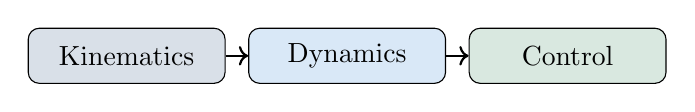
\begin{tikzpicture}[scale=0.7]
        \node[draw, rounded corners, fill=darkblue!15, minimum width=2.5cm, minimum height=0.7cm] (kin) at (0,0) {Kinematics};
        \node[draw, rounded corners, fill=brightblue!15, minimum width=2.5cm, minimum height=0.7cm] (dyn) at (4,0) {Dynamics};
        \node[draw, rounded corners, fill=darkgreen!15, minimum width=2.5cm, minimum height=0.7cm] (ctrl) at (8,0) {Control};
        
        \draw[->, thick] (kin) -- (dyn);
        \draw[->, thick] (dyn) -- (ctrl);
    \end{tikzpicture}
\end{frame}

% ============================================
% END
% ============================================
\begin{frame}
    \begin{center}
        \vspace{2cm}
        {\Huge\textbf{Questions?}}
        
        \vspace{1.5cm}
        {\large End of Lecture 4}
        
        \vspace{1cm}
        \textit{Next: Advanced Model Predictive Control (NMPC)}
    \end{center}
\end{frame}

\end{document}
